%Kompiliuoti su XeLaTeX ir BibTeX

\documentclass[a4paper, 12pt]{article}

\usepackage[yyyymmdd]{datetime}

\usepackage{fontspec}
\usepackage{fontenc}
\usepackage{ulem}
\usepackage{cite}
\usepackage{mathtools}
\usepackage{amsmath}
\usepackage{amssymb}
%\usepackage{float}
\usepackage{graphicx}
\usepackage{multirow}
\usepackage[hyphens]{url}
\usepackage{caption}
\usepackage[svgnames]{xcolor}
\usepackage{lineno}
\usepackage[lithuanian]{babel}
\usepackage{hyperref}
\usepackage{siunitx}
\usepackage{floatrow}
\usepackage[parfill]{parskip}

\floatsetup[table]{capposition=top}

\hypersetup{breaklinks=true}
\urlstyle{same}

\usepackage{geometry}
\pagestyle{myheadings}
\geometry{
	left=2cm,
	right=2cm,
	top=3cm,
	bottom=3cm,
}
\pagenumbering{arabic}
\linespread{1.25}

\graphicspath{ {images/ataskaita/} }

\renewcommand{\dateseparator}{-}
\addto\captionslithuanian{\renewcommand{\figurename}{pav}}
\addto\captionslithuanian{\renewcommand{\refname}{Literatūros sąrašas}}
\addto\captionslithuanian{\renewcommand{\tablename}{lentelė}}

\DeclareCaptionLabelFormat{numfirst}{#2~#1}
\captionsetup[figure]{labelformat = numfirst, labelsep = period}
\captionsetup[table]{labelformat = numfirst, labelsep = period}

\newcommand{\textblue}[1]{{\color{Blue}#1}}
\newcommand{\textred}[1]{{\color{Red}#1}}
\newcommand{\comment}[1]{\newline\textblue{#1}\newline}
\newcommand{\commentNL}[1]{\textblue{#1}\newline}
\newcommand{\commentMA}[1]{\textred{#1}\newline}
\newcommand{\ttt}[1]{\texttt{#1}}
\newcommand{\pT}{p_{\mathrm{T}}}
\newcommand{\ET}{E_{\mathrm{T}}}
\newcommand{\WW}{W\! W}
\newcommand{\ZZ}{Z\! Z}
\newcommand{\WZ}{W\! Z}
\newcommand{\tbarW}{\bar{t}W}
\newcommand{\ttbar}{t\bar{t}}
\newcommand{\emu}{e\mu}
\newcommand{\mumu}{\mu\mu}
\newcommand{\gJets}{\gamma\! +\!\mathrm{Jets}}
\newcommand{\WJets}{W\! +\!\mathrm{Jets}}
\newcommand{\dtW}{tW\! + \! \bar{t}W}
\newcommand{\DYee}{\mathrm{DY} \! \rightarrow \! ee}
\newcommand{\DYmumu}{\mathrm{DY} \! \rightarrow \! \mu\mu}
\newcommand{\DYtau}{\mathrm{DY} \! \rightarrow \! \tau\tau}
\newcommand{\DY}{\mathrm{DY}}
\newcommand{\ltq}[1]{{\quotedblbase{}#1\textquotedblleft{}}}
\newcommand{\Lumi}{{\cal L}_\mathrm{int}}
\newcommand{\invfb}{fb$^{-1}\,$}
\newcommand{\invpb}{pb$^{-1}\,$}
\newcommand{\QCD}{QC\! D}

\newlength\q
\setlength\q{\dimexpr .5\textwidth -2\tabcolsep}

\begin{document}
%\linenumbers

\begin{titlepage}
\centering
{\large Vilniaus universitetas \\ Fizikos fakultetas \\ Teorinės fizikos ir astronomijos institutas \par}
\vspace{3.5cm}
{\Large Marijus Ambrozas \par}
\vspace{0.3cm}
{\Large Drell-Yan proceso tyrimas analizuojant CERN CMS eksperimento 2016 metų protonų susidūrimų duomenis \par}
\vspace{0.8cm}
{\large Mokslinio darbo ataskaita \par}
\vspace{0.8cm}
%{\large Projekto nr. 09.3.3-LMT-K-712-10-0128 \par}
\vspace{3.5cm}
{\large \begin{tabular*}{0.9\textwidth}{@{\extracolsep{\fill}}ll}
Studentas & Marijus Ambrozas\tabularnewline[0.5cm]
Darbo vadovas & dr. Andrius Juodagalvis\tabularnewline[0.5cm]
\end{tabular*} \par}
\vspace{4cm}
{\large Vilnius $2019$\par}
\end{titlepage}


\clearpage
\addtocounter{page}{1}
\addtocontents{toc}{\protect\setcounter{tocdepth}{2}}
\tableofcontents
\clearpage

\section*{Įvadas} \addcontentsline{toc}{section}{Įvadas}

Protonų, sandara teoriškai yra aprašoma jų sudedamųjų dalių, vadinamų partonais, pasiskirstymo funkcijomis.
Norint suprasti hadronų greitintuvuose vykstančius procesus, kuo tikslesnis partonų pasiskirstymo funkcijų
žinojimas yra labai svarbus.
Teoriniai dviejų protonų susidūrimo metu galimų reakcijų skerspjūviai yra apskaičiuojami kaip
partonų pasiskirstymo funkcijų ir partonų tarpusavio reakcijos skerspjūvio kombinacija.
Kvantinės chromodinamikos teorija nenumato tikslių partonų pasiskirstymo funkcijų išraiškų, todėl jas bandoma
apskaičiuoti pasinaudojant įvairių procesų eksperimentinių tyrimų rezultatais \cite{NNPDF}.

Drell-Yan procesas \cite{DYoriginal} -- tai toks procesas, kai protonų susidūrimo metu kvarkas iš vieno protono ir antikvarkas
iš kito anihiliuoja sukurdami virtualų fotoną arba $Z$ bozoną, kuris netrukus skyla į leptono ir antileptono porą.
Skirtingos Drell-Yan proceso galutinės būsenos, priklausomai nuo to, kokios rūšies leptonai susidaro, yra
vadinamos kanalais: elektronų kanalas, miuonų kanalas, taonų kanalas.
Drell-Yan proceso aprašymas, naudojantis perturbacine kvantinės chromodinamika, yra gerai išplėtotas iki trečios
eilės perturbacijų tikslumo (angl.\ \textit{next-to-next-to-leading order} -- NNLO) \cite{DYNNLO}.
Ypatingai tiksliai atliekamų naujausių Drell-Yan proceso diferencialinio reakcijos skerspjūvio eksperimentinių matavimų
rezultatai pasitarnauja partonų pasiskirstymo funkcijų tikslinimui, perturbacinės kvantinės chromodinamikos bei
elektrosilpnosios sąveikos teorijų tikrinimui, taip pat ir kituose eksperimentiniuose didelių energijų fizikos
tyrimuose, kur Drell-Yan procesas yra dominuojantis triukšmas \cite{DY2018}.
Taigi, tikslūs Drell-Yan proceso matavimai yra visokeriopai svarbūs dalelių fizikos mokslui.

CERN Didysis hadronų greitintuvas vykdo labai galingus $13$ TeV energijos protonų susidūrimus \cite{DY2018}.
Egzistuoja tikimybė, kad tokių susidūrimų metu bus sukurtos nestabilios didelės masės dalelės,
kurių vidutinė gyvavimo trukmė yra labai trumpa.
Aplink protonų susidūrimo vietas išdėstytais dalelių detektoriais įmanoma užregistruoti tik tokių
dalelių skilimo produktus: fotonus, elektronus, įvairius hadronus bei miuonus.
Drell-Yan proceso tyrime ieškoma įvykių, kurių metu susidarė leptono-antileptono pora.
Egzistuoja ir taip vadinami triukšmo įvykiai, kurių galutinis produktas atrodo labai panašiai,
kaip ir galutinis Drell-Yan proceso produktas.
Kadangi paėmus vieną konkretų užregistruotą įvykį neįmanoma atskirti, ar jis yra signalo
(Drell-Yan), ar triukšmo įvykis, į triukšmų indėlį reikia atsižvelgti statistiškai įvertinant,
kokią dalį tarp visų atrinktų įvykių jie galėjo sudaryti.

Šiame darbe buvo atliekama panašių į Drell-Yan įvykių atranka bei triukšmo įvykių skaičiaus įvertinimas $\emu$ metodu.
Darbas buvo atliktas naudojant CERN CMS eksperimento 2016 metais užregistruotus protonų susidūrimų duomenis.

\section{Didysis hadronų greitintuvas ir Kompaktiškasis miuonų solenoidas}

Europos branduolinių tyrimų organizacijai CERN priklausantis Didysis hadronų greitintuvas
(angl.\ \textit{Large Hadron Collider} -- LHC) yra didžiausias ir galingiausias dalelių greitintuvas pasaulyje.
Maždaug $27$ km perimetro žiedinis greitintuvas slepiasi apytiksliai $100$ m gylyje po žeme \cite{LHC}.
Nuo $2015$ metų Didžiajame hadronų greitintuve vykstančių protonų susidūrimų energija sieka net $13$ TeV.
Įprastai jie vyksta kas $25$ ns keliuose skirtinguose žiedo taškuose, aplink kuriuose yra išdėstyti dalelių
detektoriai, priklausantys skirtingų eksperimentų grupėms.

Kompaktiškasis miuonų solenoidas (angl.\ \textit{Compact Muon Solenoid} -- CMS) yra plačios paskirties
detektorius, sukurtas įvairių skirtingų dalelių detektavimui.
CMS yra cilindrinės geometrijos detektorius, jo aukštis ir plotis -- apytiksliai po $15$ m, o ilgis --
apie $21$ m.
Detektoriaus masė siekia apie $14000$ tonų.
Detektorius susideda iš daug sluoksnių ir segmentų, kurie skirti detektuoti skirtingų rūšių dalelėms.
CMS \ltq{širdis} -- didžiausias pasaulyje solenoidinis elektromagnetas.
Tai iki superlaidumo temperatūros atšaldoma ritė, kuria darbo metu teka $19.1$ kA stiprio elektros srovė,
ir kurios viduje sukuriamas iki $4$ T siekiantis magnetinis laukas.

CMS detektoriaus segmentus galima pamatyti \ref{fig:CMSslice} paveiksle.
Kiekvienas segmentas turi vieną cilindrinę ir dvi antgalių dalis, kurios yra sluoksniškai išdėstytos
aplink protonų susidūrimo vietą.
Kiekvienas subdetektorių sluosknis yra skirtingas ir turi savo paskirtį \cite{CMSexperiment}.

Kadangi detektoriaus elektronika nėra pajėgi išsaugoti kiekvieną kas $25$ ns vykstantį įvykį, išsaugomų
įvykių skaičiui sumažinti naudojama dviejų lygių trigerių sistema \cite{CMStrig}.
Pirmojo lygio trigeris -- tai šalia detektoriaus sumontuota specialiai tam sukurta kompiuterinės
įrangos sistema.
Joje realiu laiku minimaliai apdorojami kalorimetrų bei miuonų detektorių duomenys ir pagal juos per
$4 \; \mathrm{\mu s}$ sistema nusprendžia, ar įvykis turėtų būti išrašomas tolimesnei analizei. 
Pirmojo lygio trigeris išrašo tik maždaug $1$ įvykį iš $10000$.
Aukšto lygio trigeris -- tai superkompiuterių sistema, į kurią atkeliauja pirmojo lygio trigerį
aktyvavę įvykiai.
Čia įvykiai atkuriami pasinaudojant pilna detektoriaus užregistruota informacija, bei naudojami
griežtesni atrankos kriterijai.
Tai padeda įvykių skaičių sumažinti iki maždaug $1000$ įvykių per sekundę, kurie įrašomi ilgalaikiam saugojimui,
kad vėliau galėtų būti tyrinėjami mokslininkų.

\begin{figure} \centering
	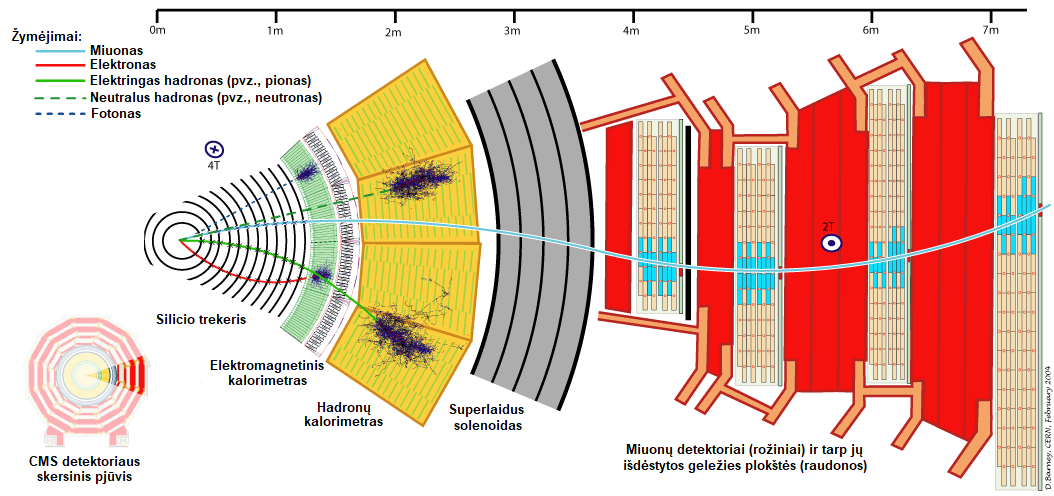
\includegraphics[width=0.95\textwidth]{CMSslice_LT.png}
	\caption{\label{fig:CMSslice}Skersinis CMS detektoriaus pjūvis \cite{CMSslice}.
	Skirtingos linijos žymi skirtingų dalelių, išlekiančių iš protonų susidūrimo vietos, trajektorijas.
	Trūki linija žymi elektriškai neutralios dalelės trajektoriją, kuri silicio trekų detektoriuje
	neužfiksuojama.}
\end{figure}

\section{Duomenų rinkiniai}

Šiame darbe buvo naudojami dalinai apdoroti CERN CMS detektoriaus 2016 metais užregistruoti $13$ TeV
energijos protonų susidūrimų duomenys, atitinkantys $35.9$ \invfb integruotąjį šviesį.
Tai yra virš $10$ kartų daugiau protonų susidūrimų, nei užregistruota $2015$-aisiais metais \cite{DY2018}.

Taip pat darbe buvo naudojami modeliuoto Drell-Yan signalo ir pagrindinių triukšmo procesų duomenų rinkiniai.
Drell-Yan signalo bei $\WJets$ proceso duomenų rinkiniai buvo sumodeliuoti naudojant
\ttt{MadGraph5\_aMC@NLO} įvykių modeliavimo programą \cite{MG_aMCatNLO}.
Viršūninio-antiviršūni-nio kvarko poros ($t\bar{t}\,$) ir vieno viršūninio kvarko kartu su $W$ bozonu ($tW$ arba
$\bar{t}W$) įvykiai buvo sumodeliuoti naudojant \textsc{Powheg} \cite{powheg_ttbar, powheg_tW}.
Visi šie išvardinti procesai buvo sumodeliuoti antros eilės perturbacijų tikslumu (angl.
\textit{next-to-leading order} -- NLO).
Dviejų bozonų ($WW$, $WZ$, $ZZ$) įvykiai buvo sumodeliuoti su \textsc{Pythia8} pirmos eilės perturbacijų tikslumu
(angl. \textit{leading order} -- LO) \cite{pythia82}.
Detektoriaus atsakas į kiekvieną iš sumodeliuotų įvykių buvo modeliuojamas naudojantis \textsc{Geant4} programa
\cite{geant4}.

Visi naudoti duomenys saugomi Pietų Korėjos Tier2 duomenų centre ir užima apie $14$ TB.
Duomenų analizė buvo vykdoma dviem etapais: pirmiausia buvo atliekama įvykių atranka nuotoliniu būdu prisijungus
prie skaičiavimo centro.
Svarbiausia su atrinktais įvykiais susijusi informacija buvo įrašoma į naujus duomenų failus, kurie užima tik
apie $8$ GB.
Naujai sukurti failai buvo parsisiunčiami į vietinį kompiuterį tolimesnei analizei.


\section{Įvykių atranka}\label{sec:selection}
Iš $2016$-aisiais metais CMS detektoriaus užregistruotų duomenų buvo stengiamasi išrinkti tokius įvykius, kurie
su kuo didesne tikimybe atitiktų Drell-Yan procesą.
Drell-Yan proceso miuonų galutinei būsenai buvo naudojamas vieno miuono trigeris, kuris aktyvuojamas tada,
kai aptinkamas bent vienas miuonas su skersiniu impulsu, didesniu, nei $24$ GeV.
Miuonas gali būti atpažintas pasinaudojant tiek trekų detektoriaus, tiek miuonų detektoriaus informacija.
Toliau kiekvienam miuonui buvo taikomi \ttt{TightID} reikalavimai \cite{MuonID}, kurie skirti sumažinti atranką
praeinančių netikrų miuonų, bei miuonų, atsiradusių iš antrinių procesų, skaičių.
Taip pat kiekvienam miuonui buvo taikomas trajektorijos izoliuotumo reikalavimas: pašalinių dalelių, aptiktų
$\Delta R = \sqrt{(\Delta\eta)^2 + (\Delta\phi)^2} < 0.3$ (čia $\eta$ -- pseudosparta, $\phi$ -- sferinės koordinačių
sistemos azimutinis kampas) pločio kūgyje, nubrėžtame aplink miuono trajektoriją, skersinių impulsų suma negali
viršyti $15\%$ miuono skersinio impulso vertės.
Tolimesnis kriterijus buvo toks, kad miuonų poros trajektorijas pakankamai tiksliai eitų suvesti į vieną pirminę
viršūnę bei kad abu miuonai būtų priešingų elektrinių krūvių.
Tam, kad būtų išvengta miuonų iš kosminės spinduliuotės aptikimo, buvo taikomas papildomas kriterijus, reikalaujantis,
kad kampas tarp dviejų miuonų trajektorijų būtų mažesnis, nei $\pi-0.005$ rad.

Elektronų galutinei būsenai buvo naudojamas dviejų elektronų trigeris, kuris aktyvuojamas tada, kai aptinkami
bent du elektronai, vieno iš kurių skersinis impulsas didesnis, nei $23$ GeV, o kito -- didesnis nei $12$ GeV.
Kiekvienam elektronui buvo taikomi \ttt{MediumID} reikalavimai (idėja aprašyta \cite{EleID}, tačiau tikslios
reikalavimų vertės skiriasi nuo naudotų darbe, nes jos yra atnaujinamos CMS vidiniuose dokumentuose), kurie
skirti sumažinti elektronų, atsiradusių fotono virsmo į elektrono-pozitrono porą metu, bei netikrų elektronų
skaičių.
Taip pat buvo reikalaujama, kad elektronai nepatektų į sritį $1.4442<|\eta_{\mathrm{SC}}|<1.566$, nes joje
yra perėjimas iš elektromagnetinio kalorimetro cilindrinės į antgalio dalį ir dėl ten išvedžiotos elektronikos
detektavimo efektyvumas šioje srityje nėra toks geras.

Galiausiai tiek elektronai, tiek miuonai turėjo praeiti tokius pačius kinematinius atrankos kriterijus,
reikalaujančius, kad greitesnysis leptonas iš dviejų turėtų skersinį impulsą, didesnį už $28$ GeV, o lėtesnysis --
didesnį už $17$ GeV bei kad abiejų leptonų pseudospartų absoliutinės vertės neviršytų $2.4$.
Jei tokią atranką praeitų kelios miuonų poros, iš jų išrenkama ta pora, kurių trajektorijas galima suvesti į
vieną pirminę viršūnę didžiausiu tikslumu.

Pagrindinis matuojamas dydis buvo atranką praėjusių leptonų porų invariantinė masė.
Iš jų buvo brėžiama invariantinės masės histograma, apimanti masės sritį nuo $15$ iki $3000$ GeV.


\section{Pataisos}\label{sec:corrections}
Kad būtų galima palyginti matavimą su modeliavimu, modeliuotų įvykių skaičius turi būti sunormuotas
į išmatuotą integruotąjį šviesį.
Tai daroma kiekvienam modeliuotam įvykiui priskiriant svorį, kuris apskaičiuojamas pagal tokią formulę:
\begin{equation}
	\omega_{i}^{\mathrm{Piln.}} = \omega_{i} \frac{ \sigma\Lumi }{ \sum_{i=j}^{N}\omega_{j} } \; ,
	\label{eq:NLOweight}
\end{equation}
čia $\omega_{i}$ kiekvieno įvykio individualus svoris, priskirtas įvykių modeliavimo programos,
$\sigma$ -- tam tikro proceso (pvz., Drell-Yan) reakcijos skerspjūvis, $N$ -- įvykių skaičius to
proceso modeliuotų duomenų rinkinyje, $\Lumi$ -- išmatuotas integruotasis šviesis.

\vspace{0.5cm}
\begin{minipage}[t]{0.48\textwidth}
	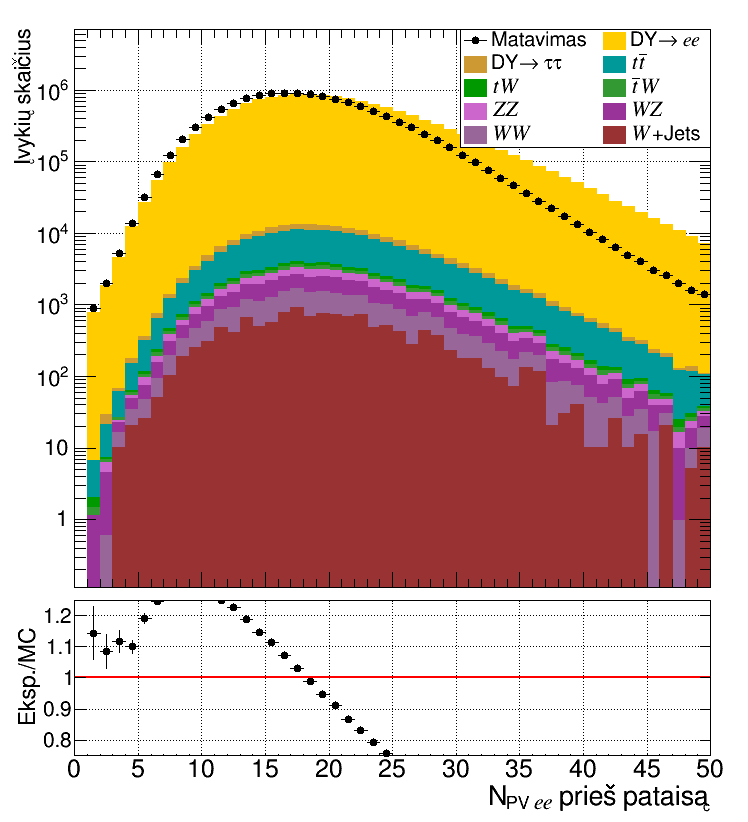
\includegraphics[width=\linewidth]{nVTXee_before.png}
\end{minipage}
\hfill
\begin{minipage}[t]{0.48\textwidth}
	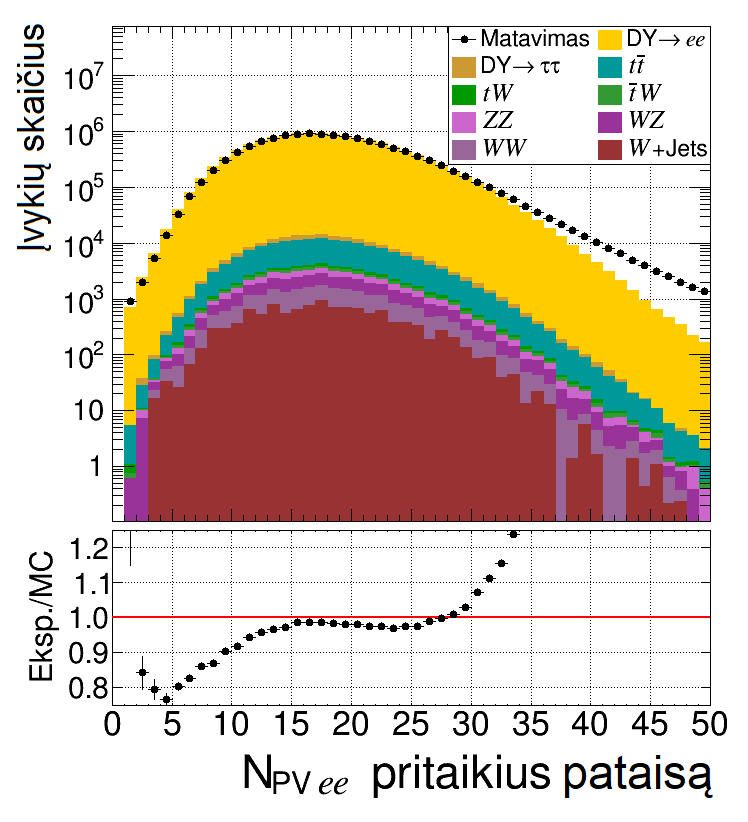
\includegraphics[width=\linewidth]{nVTXee_after.png}
\end{minipage}
\vspace{-0.9cm}
\captionof{figure}{\label{fig:PUba} Pirminių viršūnių skaičiaus pasiskirstymai atranką praėjusiuose elektronų poros
		įvykiuose prieš (kairėje) ir po (dešinėje) pataisos pritaikymo.
		Juodi taškai vaizduoja CMS detektoriumi išmatuotą, o spalvoti stulpeliai -- modeliuotus pasiskirstymus.}
\vspace{0.5cm}

Įprastai per vieną protonų spindulio porcijų prasikeitimą (angl.\ \textit{bunch crossing}) susiduria
daugiau negu viena protonų pora ir tai turi įtakos užregistruoto įvykio atkūrimo kokybei.
Šį efektą bandoma simuliuoti modeliuotuose įvykiuose, tačiau dažniausiai tikimybinis protonų susidūrimų
skaičiaus (per vieną prasikeitimą) pasiskirstymas matavime ir modeliavime nesutampa.
Šį nesutapimą bandoma sumažinti taikant protonų susidūrimo skaičiaus pataisas -- kiekvienam modeliuotam
įvykiui priskiriamas tam tikras svoris pagal tai, koks protonų susidūrimų skaičius jame buvo sumodeliuotas.
Pataisa buvo taikoma darant prielaidą, kad protonų susidūrimo skerspjūvis greitintuve yra lygus $64$ mb.
Išmatuoti ir modeliuoti atkurtų pirminių viršūnių skaičiaus pasiskirstymai elektronų poros įvykiuose
prieš ir po pataisos pateikiami \ref{fig:PUba} pav.
Miuonų poros įvykiams grafikų forma yra analogiška, tik skiriasi suminis įvykių skaičius.

Paveikslų apatinėse dalyje pateiktuose eksperimentinio ir modeliuoto rezultatų santykio grafikuose galima pamatyti, kad
$10$-$30$ pirminių viršūnių skaičiaus srityje, į kurią patenka apie $91\%$ visų įvykių, grafikai tampa plokštesni --
šioje srityje pirminių viršūnių skaičiaus pasiskirstymai sutampa labai gerai.

Elektronų poros invariantinės masės matavimo kokybei įtakos turi elektronų energijos matavimo
tikslumas, o miuonų poros invariantinei masei -- miuonų skersinio impulso matavimo tikslumas.
Dėl to visiems užregistruotiems elektronams buvo pritaikytos standartinės CMS elektronų energijos skalės
pataisų procedūros \cite{Ecorr}, o miuonams -- Ročesterio mokslinės grupės pateikiamos miuonų impulso
skalės pataisos \cite{RocCorr}.

Kadangi dėl modeliavimo netobulumo nesutapo tam tikros realaus ir virtualaus eksperimento sąlygos,
kiekvienam elektronų poros įvykiui buvo priskiriami svoriniai daugikliai, priartinantys modeliuotus trigerių
suveikimo ir elektrono trajektorijos atkūrimo bei atpažinimo efektyvumus prie išmatuotųjų.
Miuonų poros įvykiams buvo priskirti daugikliai, atsižvelgiantys į trigerių bei miuonų trajektorijos atkūrimo,
atpažinimo ir izoliuotumo įvertinimo efektyvumų nesutapimus.
Kiekvieno daugiklio vertės buvo nustatomos pagal leptono skersinio impulso ir pseudospartos vertes.
Invariantinės masės pasiskirstymai prieš ir po šių pataisų pritaikymo pateikiami \ref{fig:invMb} ir
\ref{fig:invMa} pav.
Palyginus paveikslų apačioje pateikiamus matavimo ir modeliavimo santykio pasiskirstymus galima pamatyti, kad
pritaikius minėtas pataisas sutapimas tarp eksperimento ir modeliavimo pagerėjo vidutiniškai apie $10\%$.

\vspace{0.5cm}
\begin{minipage}[t]{0.48\textwidth}
	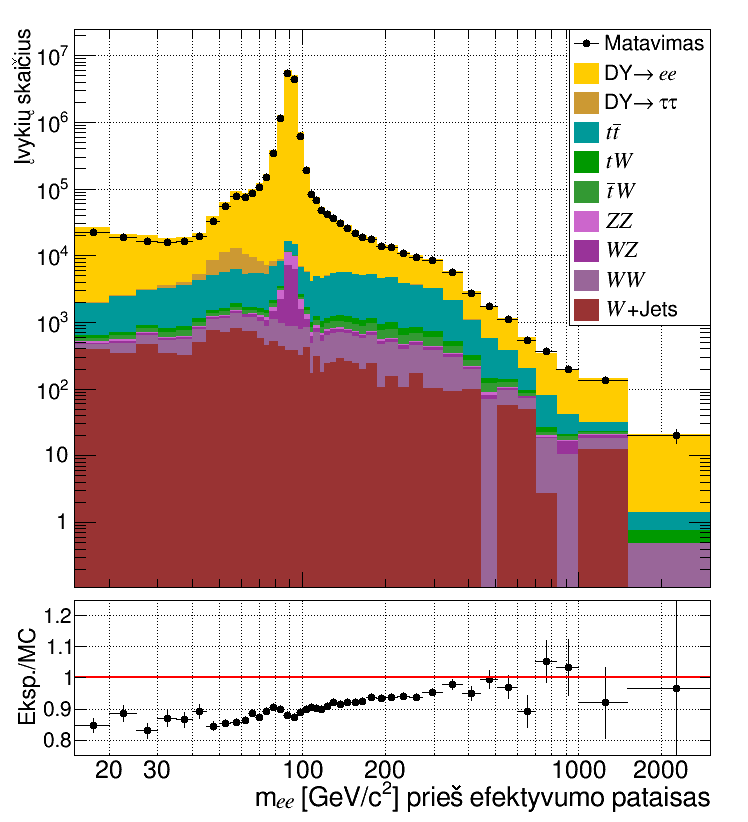
\includegraphics[width=\linewidth]{ee_mass_beforeSF.png}
\end{minipage}
\hfill
\begin{minipage}[t]{0.48\textwidth}
	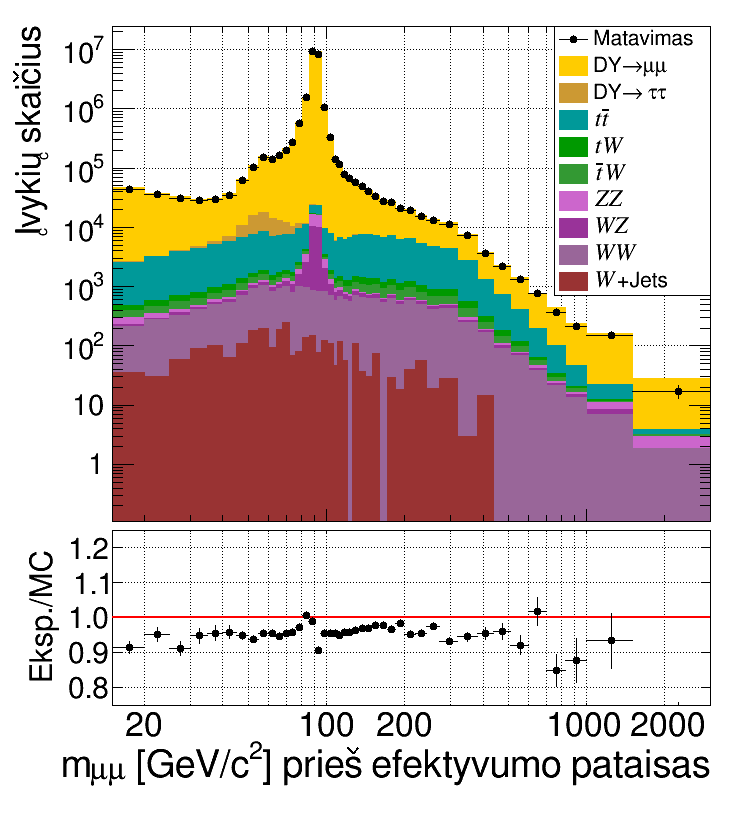
\includegraphics[width=\linewidth]{mumu_mass_beforeSF.png}
\end{minipage}
\vspace{-0.9cm}
\captionof{figure}{\label{fig:invMb} Elektronų (kairėje) ir miuonų (dešinėje) porų invariantinės masės pasiskirstymai
		prieš efektyvumo pataisų pritaikymą.}
\vspace{0.5cm}


Yra pastebėta, kad antros eilės perturbacijų tikslumu modeliuojant viršūninių kvarkų poros ($t\bar{t}\,$)
įvykius, gaunami modeliuoti viršūninių kvarkų skersinių impulsų pasiskirstymai turi nesutapimų su nustatytais
iš eksperimento \cite{ttbarPT}.
Kadangi $t\bar{t}$ yra vienas iš Drell-Yan triukšmo procesų, norint turėti kuo tikslesnį triukšmo įvertį, į šį
modeliavimo trūkumą svarbu atsižvelgti.
Tai buvo daroma modeliuotiems viršūninių kvarkų poros įvykiams priskiriant papildomus svorius, kurie skirti
priartinti modeliuotą kvarkų skersinių impulsų pasiskirstymą prie naujausių eksperimentinių rezultatų.
Svorių vertės nustatomos pagal kvarkų skersinių impulsų vertes.

\vspace{0.5cm}
\begin{minipage}[t]{0.48\textwidth}
	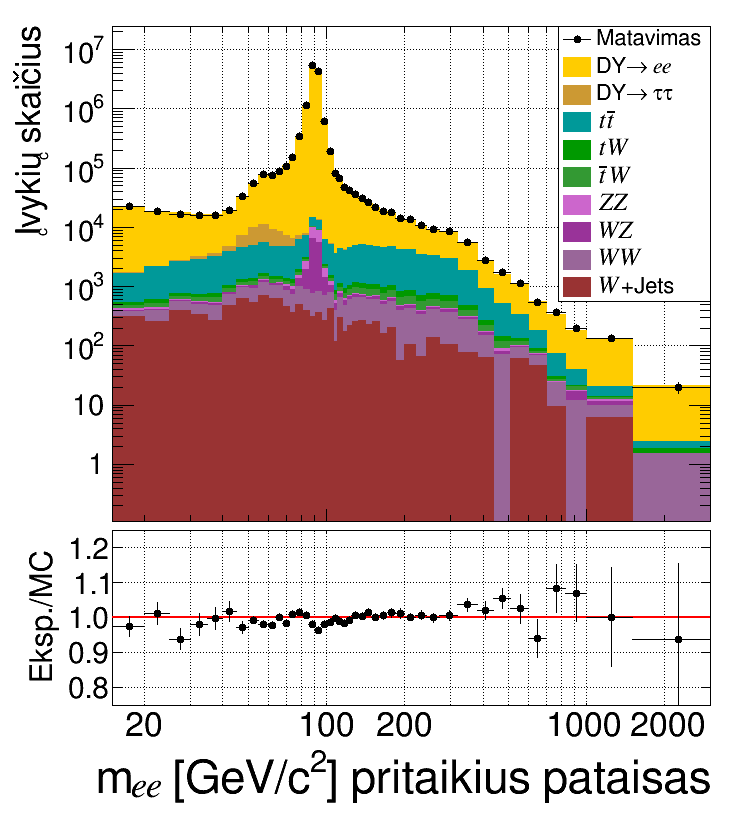
\includegraphics[width=\linewidth]{ee_mass_after.png}
\end{minipage}
\hfill
\begin{minipage}[t]{0.48\textwidth}
	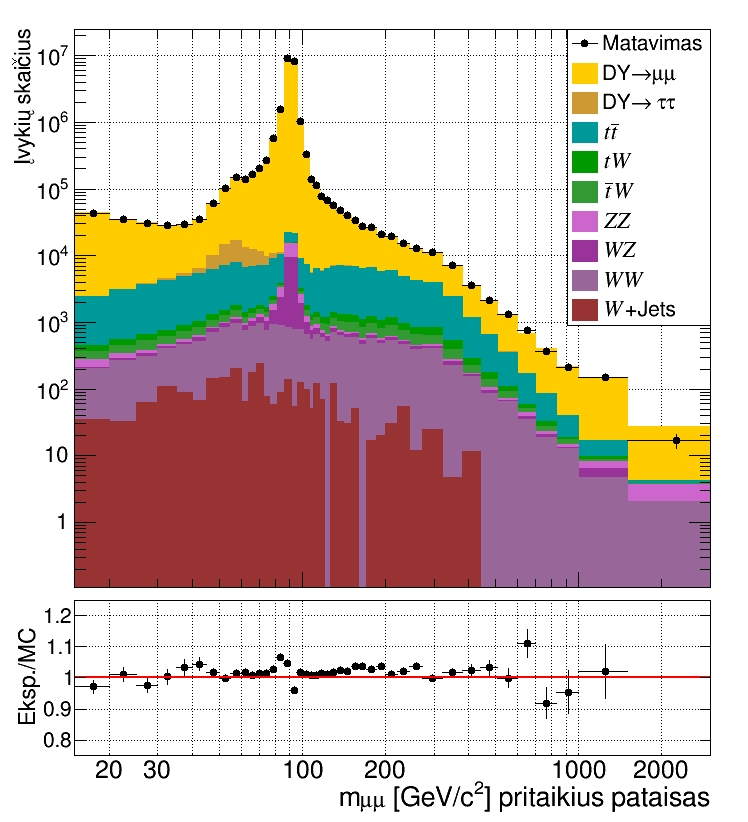
\includegraphics[width=\linewidth]{mumu_mass_after.png}
\end{minipage}
\vspace{-0.9cm}
\captionof{figure}{\label{fig:invMa} Elektronų (kairėje) ir miuonų (dešinėje) porų invariantinės masės pasiskirstymai,
		gauti pritaikius efektyvumo pataisas.}
\vspace{0.5cm}


Taip pat dėl eksperimentinio ir modeliuoto leptonų pseudospartos bei leptonų poros spartos pasiskirstymų nesutapimų
buvo taikomos dar dvi pataisos.
Viena pataisa buvo skirta ištaisyti protonų susidūrimo vietos $z$ koordinatės ($z$ ašis eina išilgai protonų
spindulio lėkimo krypties detektoriaus centre) nesutapimus tarp matavimo ir modeliavimo.
Tai padėjo sumažinti \ref{fig:rapibPVZ} pav.\ apačioje esančiuose matavimo ir modeliavimo santykio pasikirstymuose
matomus asimetriškumus.
Kita pataisa buvo reikalinga todėl, kad darbe naudotų duomenų registravimo laikotarpiu buvo susidurta su problema,
kai tam tikru atveju trigerio suveikimas buvo priskiriamas ne tam įvykiui, kuris iš tikrųjų jį aktyvavo, o
ankstesniam.
Dėl šio efekto dalis įdomių įvykių, kuriuose sukurtos dalelės turėjo dideles pseudospartos vertes ($|\eta|>2$)
liko neįrašyti.
Imituoti šiam pernelyg ankstyvo trigerio suveikimo efektui buvo pritaikyta pataisa, kuri priskirdavo įvykiams
svorius pagal tai, kiek ir kokių įvykyje užregistruotų objektų patenka į didesnių pseudospartų sritį.
Tai turėjo įtakos ir leptonų poros spartos pasiskirstymui: palyginus \ref{fig:rapibL1} su \ref{fig:rapia} pav.\
galima matyti, kad pataisos pritaikymas padėjo sumažinti modeliuotų įvykių skaičių ties didesnėmis spartos modulio
vertėmis ir priartino modeliuotus rezultatus prie išmatuotųjų.

\vspace{0.25cm}
\begin{minipage}[t]{0.48\textwidth}
	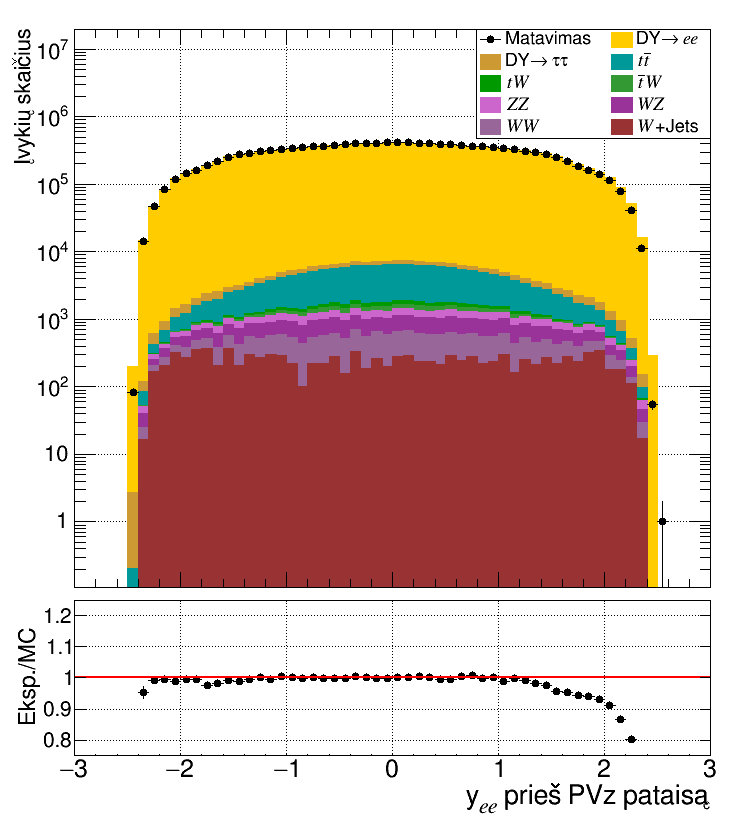
\includegraphics[width=\linewidth]{ee_rapi_beforePVZ.png}
\end{minipage}
\hfill
\begin{minipage}[t]{0.48\textwidth}
	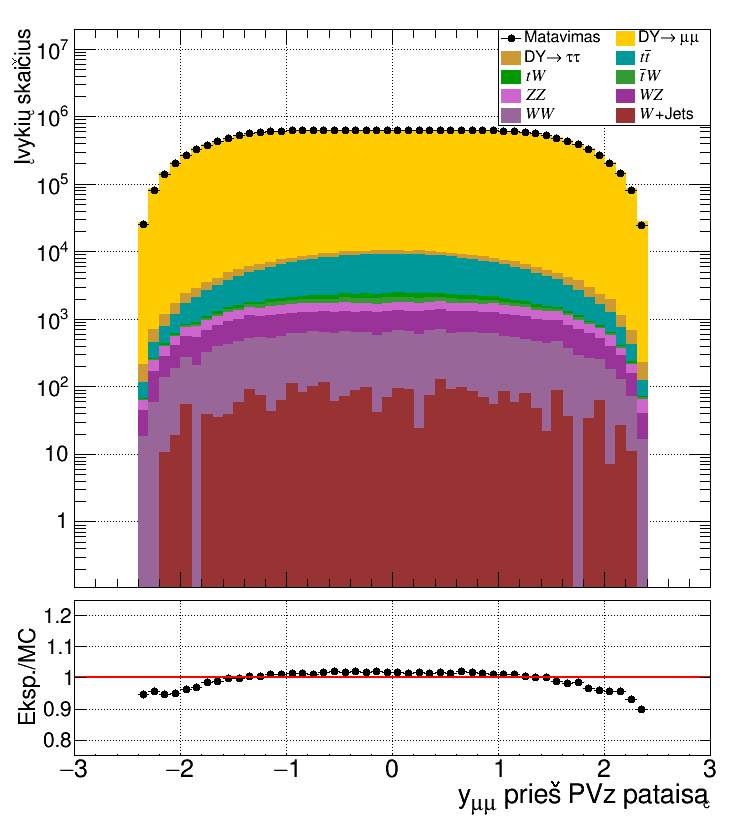
\includegraphics[width=\linewidth]{mumu_rapi_beforePVZ.png}
\end{minipage}
\vspace{-0.9cm}
\captionof{figure}{\label{fig:rapibPVZ} Elektronų (kairėje) ir miuonų (dešinėje) porų spartos pasiskirstymai
		prieš pirminės viršūnės $z$ koordinatės pataisos pritaikymą.
		Atkreiptinas dėmesys į eksperimento ir modeliavimo santykio pasiskirstymo asimetriškumą.}

\vspace{1.5cm}
\begin{minipage}[t]{0.48\textwidth}
	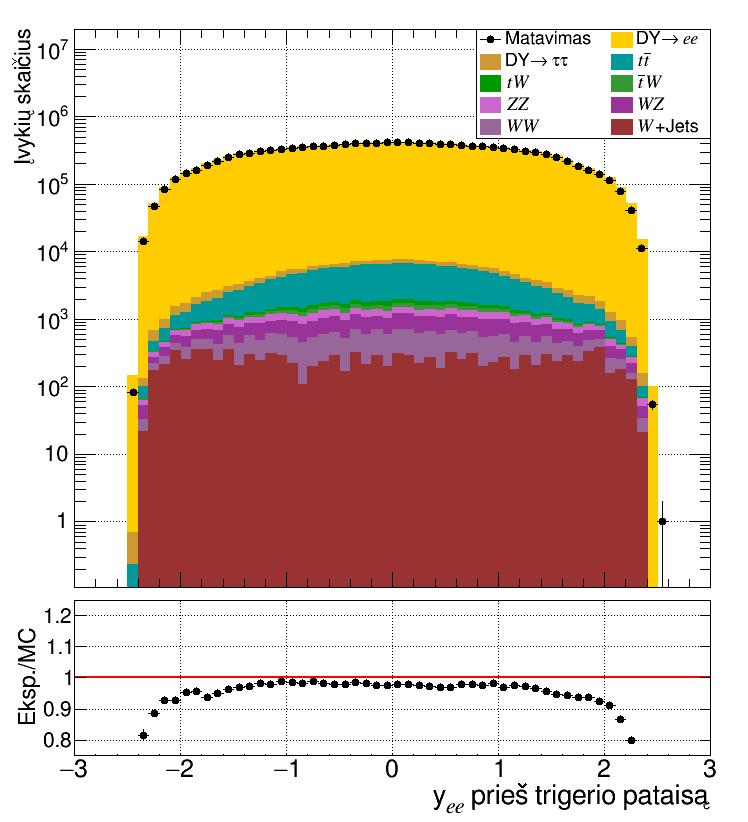
\includegraphics[width=\linewidth]{ee_rapi_beforeL1.png}
\end{minipage}
\hfill
\begin{minipage}[t]{0.48\textwidth}
	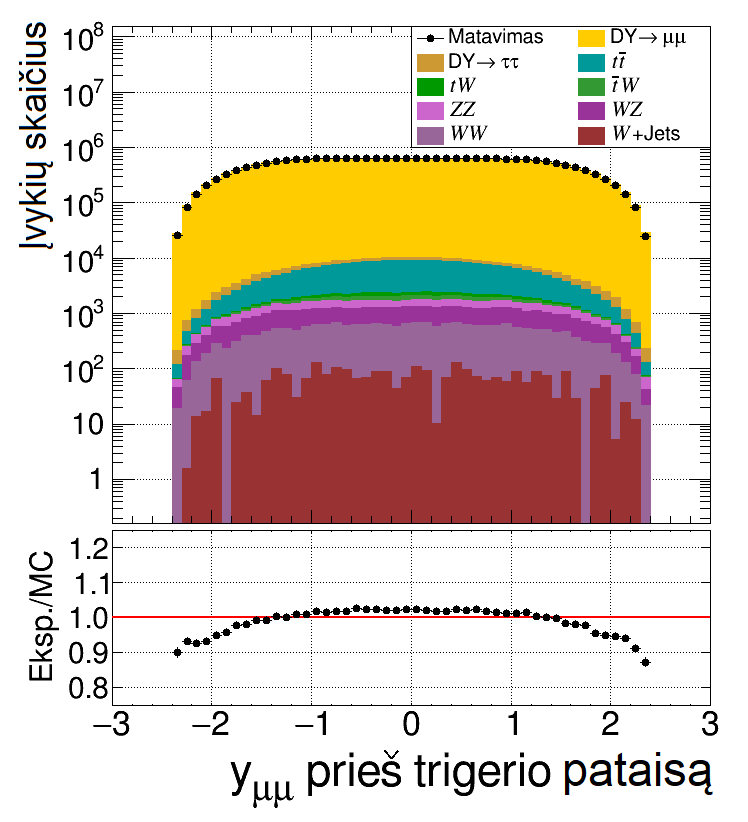
\includegraphics[width=\linewidth]{mumu_rapi_beforeL1.png}
\end{minipage}
\vspace{-0.9cm}
\captionof{figure}{\label{fig:rapibL1} Elektronų (kairėje) ir miuonų (dešinėje) porų spartos pasiskirstymai,
		gauti po pirminės viršūnės $z$ koordinatės pataisos pritaikymo, tačiau dar nepritaikius per ankstaus
		trigerio suveikimo pataisos.}

\vspace{0.25cm}
\begin{minipage}[t]{0.48\textwidth}
	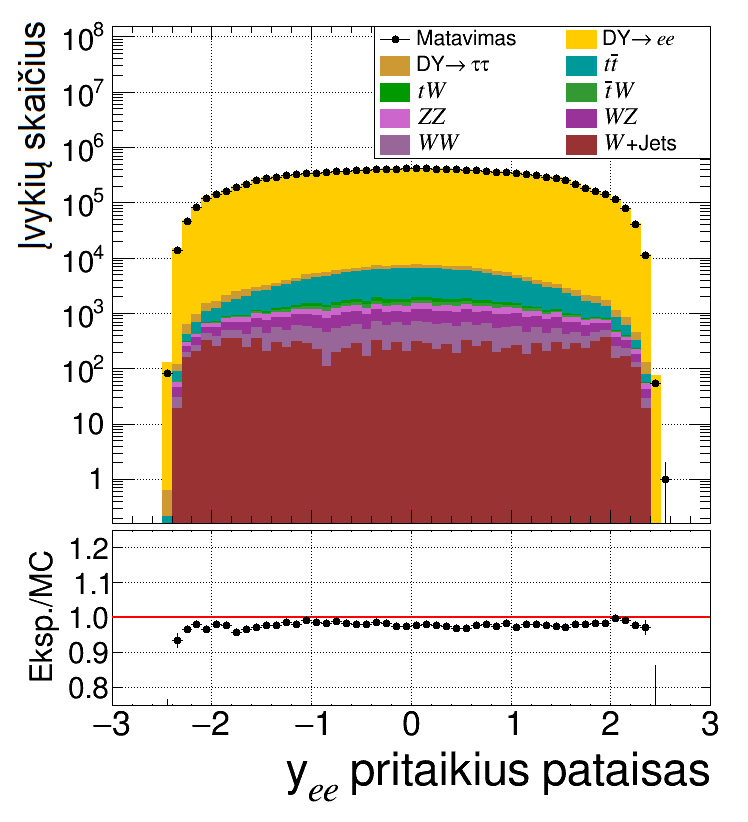
\includegraphics[width=\linewidth]{ee_rapi_after.png}
\end{minipage}
\hfill
\begin{minipage}[t]{0.48\textwidth}
	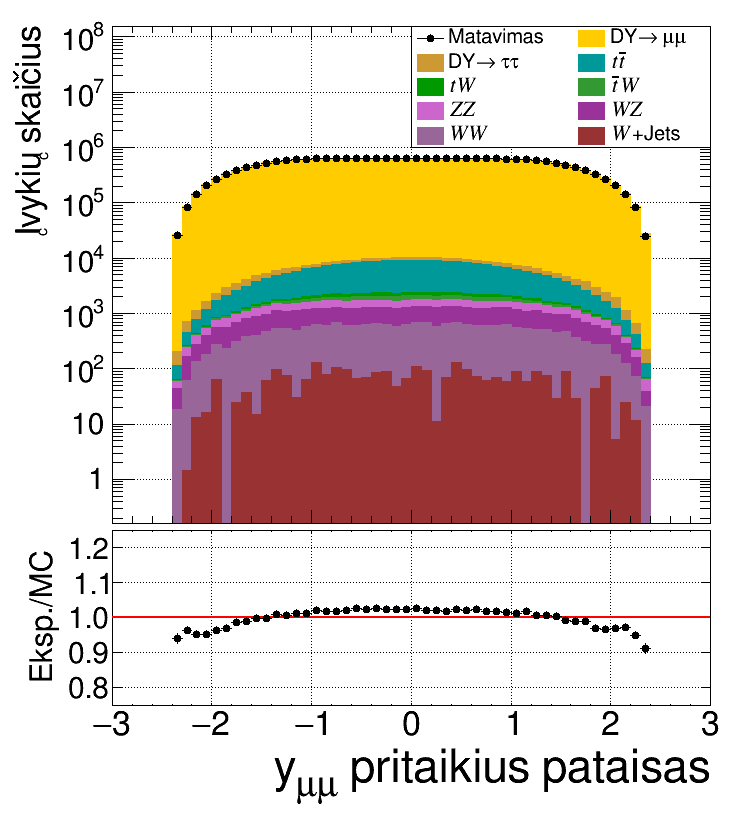
\includegraphics[width=\linewidth]{mumu_rapi_after.png}
\end{minipage}
\vspace{-0.9cm}
\captionof{figure}{\label{fig:rapia} Elektronų (kairėje) ir miuonų (dešinėje) porų spartos pasiskirstymai,
		gauti pritaikius visas pataisas.}
\vspace{-0.2cm}


\section{Triukšmų indėlio įvertinimas}\label{sec:SignalBkg}
	 
Pagrindiniai Drell-Yan proceso triukšmai yra šie: viršūninių kvarkų poros ($t\bar{t}\,$) įvykiai, dviejų bozonų
įvykiai ($WW$, $WZ$ ir $ZZ$), vieno viršūninio kvarko ir $W$ bozono įvykiai ($tW$ arba $\bar{t}W$), $W$ bozono
ir čiurkšlės įvykiai ($\WJets$) bei stipriosios sąveikos nulemti kelių čiurkšlių įvykiai (sutrumpintai vadinami $\QCD$).
Taip pat tiriant Drell-Yan proceso elektronų ir miuonų kanalus vienas iš svarbių triukšmų yra
to paties Drell-Yan proceso taonų kanalas (taonai skyla į elektronus arba miuonus) $\DYtau$.
Pagrindiniai būdai triukšmo įvykių skaičiaus įvertinimui yra Monte Carlo (MC) modeliavimas ir
matavimu grįsti metodai.

Monte Carlo modeliavimas -- tai toks metodas, kai tikimybiniu pasiskirstymu aprašomo
įvykio baigtis sumodeliuojama generuojant atsitiktinius skaičius.
Tokį virtualų eksperimentą kartojant daug kartų galima gauti rezultatą, kuris yra palyginamas
su eksperimentu (kur fiksuojama tam tikra užregistruotų įvykių statistika).
Vis dėlto, sumodeliuoti įvykius taip, kad virtualaus eksperimento sąlygos idealiai atitiktų
realaus eksperimento sąlygas, yra praktiškai neįmanoma.
Dėl to modeliuotiems įvykiams reikia taikyti į kai kuriuos iš neatitikimų atsižvelgiančias pataisas.
Tačiau vis tiek egzistuoja neapibrėžtumų, tokių, kaip nepakankamos žinios apie atskirų triukšmo
procesų įvykių tikėtinumus, neidealus detektoriaus atsako modeliavimas ir pan., kurie kenkia
įverčio kokybei.
Šių problemų gali būti išvengiama triukšmo įvykių skaičiaus įvertinimui naudojant matavimu
grįstus metodus.

Matavimu grįsti metodai apjungia matavimą ir modeliavimą, kad būtų gautas kuo
tikroviškesnis įvykių skaičiaus įvertis.
Pagrindinis matavimu grįstų įvykių skaičiaus įvertinimo metodų principas remiasi signalo ir
kontrolinės sričių apibrėžimais.
Signalo sritis -- tai sritis, pasirinkta taip, kad į ją patektų
kuo daugiau signalo ir kuo mažiau triukšmo įvykių.
Kontrolinė sritis -- tai taip pasirinkta sritis, kad į ją patektų kuo daugiau triukšmo ir kuo
mažiau signalo įvykių.
Skirtingi matavimu grįsti metodai yra būdai transformuoti triukšmo įvykių skaičių, apskaičiuotą
kontrolinėje srityje, į triukšmo įvykių skaičių, patenkantį į signalo sritį.
Eksperimentinėje didelių energijų fizikoje ganėtinai populiarūs yra klaidingo atpažinimo ir ABCD metodai.
Jie naudojami įvertinti skaičiui tokių triukšmo įvykių, kurių metu susidarė čiurkšlės.
Triukšmų, siejamų su procesais, kurių metu susidariusios dvi nestabilios dalelės skyla
į leptonus nepriklausomai ir su vienodomis tikimybėmis, indėliui įvertinti naudojamas $\emu$ metodas,
kuris ir buvo taikomas šiame darbe.

$\emu$ metodas buvo naudojamas įvertinti triukšmus, siejamus su $\DYtau$, $t\bar{t}\,$, $WW$,
$tW$, $\bar{t}W$ procesais.
Kitų triukšmo procesų indėlis buvo įvertintas iš modeliavimo, išskyrus $QCD$ įvykius, kurių modeliavimas
neaprašo pakankamai gerai.
Ateityje $QCD$ indėlis bus įvertintas klaidingo atpažinimo metodu, o į dabartinį tyrimą jis nebuvo įtrauktas.

Taikant $\emu$ metodą signalo sritis apibrėžiama pagal \ref{sec:selection} skyriuje aprašytus kriterijus.
Kontrolinė sritis apibrėžiama pagal panašius kriterijus, tačiau galutinėje būsenoje ieškome
ne dviejų elektronų ar dviejų miuonų, o vieno elektrono ir vieno miuono.
Tokios būsenos neįmanoma gauti iš Drell-Yan proceso signalo, taigi joje bus vien triukšmo įvykiai.
Triukšmo įvykių skaičius iš kontrolinės srities ($\emu$) į signalo sritį ($ee$ arba $\mu\mu$)
transformuojamas pasinaudojant Monte Carlo modeliavimu:

\begin{equation}
	N_{ee}^{\mathrm{Tr. \, įvert.}} =
	\frac{ N_{ee}^{\mathrm{Tr. \, MC}} }{ N_{e\mu}^{\mathrm{Tr. \, MC}} }
	\cdot N_{e\mu}^{\mathrm{Tr. \, eksp.}} \; ,
	\label{eq:emuMethod}
\end{equation}
čia $N_{ee}^{\mathrm{Tr. \, įvert.}}$ -- $\emu$ metodu įvertintas triukšmo įvykių skaičius signalo
(šiuo atveju, $ee$) srityje, $N_{e\mu}^{\mathrm{Tr. \, eksp.}}$ -- išmatuotas įvykių skaičius
kontrolinėje srityje, $N_{ee}^{\mathrm{Tr. \, MC}}$ ir $N_{e\mu}^{\mathrm{Tr. \, MC}}$ -- modeliuotų
triukšmo įvykių skaičiai atitinkamai signalo ir kontrolinėje srityje.

Elektrono ir miuono galutinės būsenos įvykiai buvo atrenkami kombinuojant $ee$ ir $\mu\mu$ atrankos
kriterijus -- elektronui buvo taikomi $ee$ atrankoje naudoti, o miuonui -- $\mu\mu$ atrankoje naudoti
kriterijai, tik šiai atrankai buvo naudotas vieno miuono trigeris (nenaudota elektronų trigerių).
Šiems įvykiams buvo pritaikytos ir visos \ref{sec:corrections} skyriuje aprašytos pataisos.

Kadangi $\emu$ įvykių atranką praeina ir ganėtinai reikšminga netikrų $\emu$ įvykių dalis (pagrinde
$W+\mathrm{Jets}$ ir $QCD$ įvykiai, kuriuose čiurkšlė būna klaidingai atpažinta kaip leptonas),
norint kaip įmanoma tiksliau įvertinti Drell-Yan proceso triukšmus, pirmiausia reikia
įvertinti netikrų $\emu$ įvykių skaičių.
$QCD$ indėlis buvo įvertintas dar vienu matavimu grįstu metodu.
Šiuo atveju signalo sritis buvo $\emu$ įvykiai, kuriuose elektronas ir miuonas yra priešingų elektrinių
krūvių, o kontrolinė sritis -- įvykiai, kuriuose elektrono ir miuono krūviai yra vienodi.
$QCD$ įvykių skaičius iš kontrolinės srities į signalo sritį buvo perkeliamas padalinant jį iš
konstantos $R\approx 0.57$, kuri apskaičiuojama teoriškai, padarius prielaidą, kad visi atranką
praeinantys $QCD$ įvykiai yra giluminių kvarkų poros ($b\bar{b}$) įvykiai.
Šios procedūros veikimo principas yra pavaizduotas \ref{fig:emuQCD} pav.
$W+\mathrm{Jets}$ indėlis buvo įvertintas iš modeliavimo.
Prieš taikant $\emu$ metodą gautas netikrų $QCD$ įvykių skaičiaus įvertis buvo atimtas iš
$N_{e\mu}^{\mathrm{Tr. \, eksp.}}$, o $W+\mathrm{Jets}$ indėlis buvo įskaitytas sumažinant
$N_{e\mu}^{\mathrm{Tr. \, eksp.}}$ dydžiu $1/1+C$, kur
\begin{equation*}
	C = \frac{ N_{W+\mathrm{Jets}}^{\mathrm{MC}} } { N_{\mathrm{DY}\rightarrow\tau\tau}^{\mathrm{MC}} + 
	N_{t\bar{t}}^{\mathrm{MC}} + N_{WW}^{\mathrm{MC}} + N_{WZ}^{\mathrm{MC}} + N_{tW}^{\mathrm{MC}} + N_{\bar{t}W}^{\mathrm{MC}} +
	N_{ZZ}^{\mathrm{MC}} + N_{W+\mathrm{Jets}}^{\mathrm{MC}} } \; ,
\end{equation*}
čia $N^{\mathrm{MC}}_{...}$ -- modeliuotų tam tikro proceso $\emu$ galutinės būsenos įvykių skaičius.

\begin{figure}[H]
	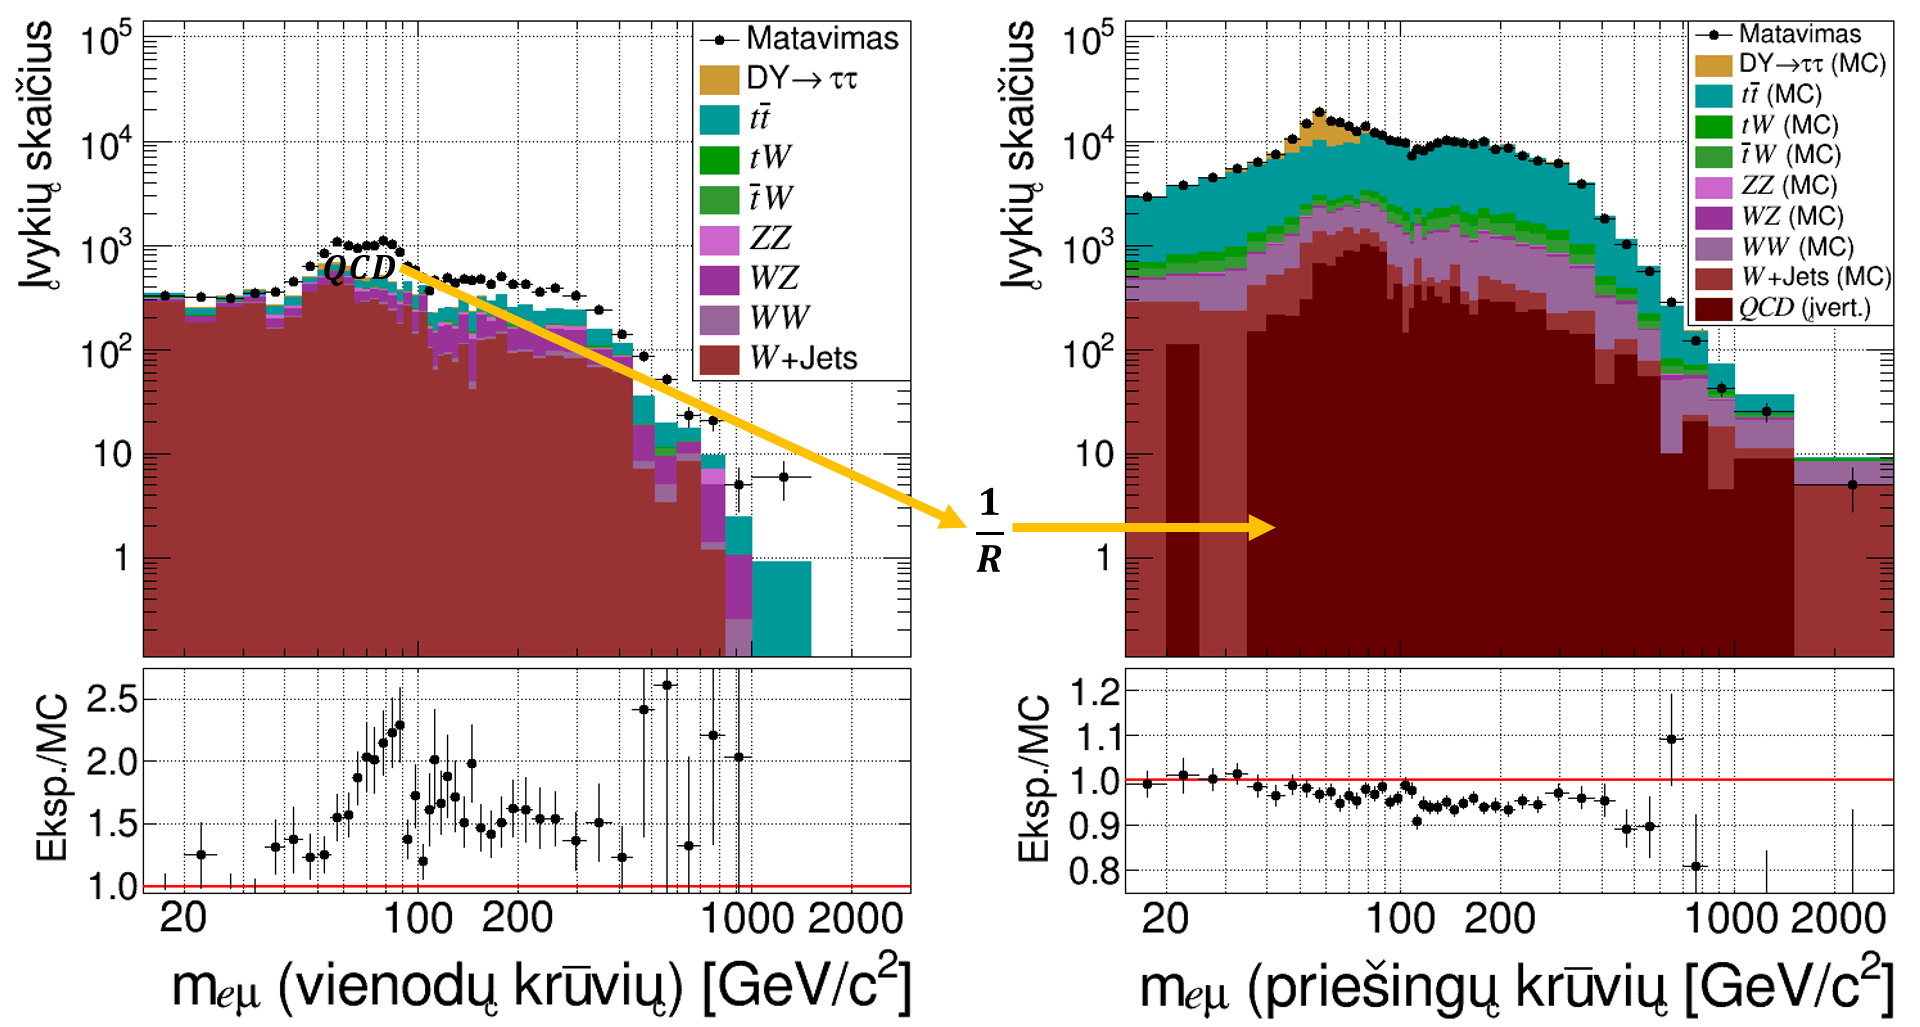
\includegraphics[width=0.95\textwidth]{emuQCDest.png}
	\vspace{-0.2cm}
	\caption{\label{fig:emuQCD} Vienodą (kairėje) ir priešingą (dešinėje) krūvį turinčių elektrono ir
	miuono invariantinės masės pasiskirstymai.
	Kairiajame grafike matomas didžiulis skirtumas tarp eksperimentinio ir modeliuoto rezultato buvo
	priskirtas su $QCD$ procesu siejamiems netikriems $\emu$ įvykiams.
	$QCD$ įvykių skaičius iš vienodų krūvių (kontrolinės) srities į priešingų krūvių (signalo) sritį
	buvo transformuotas padalinus jį iš konstantos $R$.}
\end{figure}

\section{Paklaidų įvertinimas}\label{sec:uncertainties}

Statistinė įvykių skaičiaus paklaida kiekvienam histogramos stulpeliui buvo skaičiuojama kaip visų
į jį patenkančių įvykių svorių kvadratų suma:
\begin{equation}
	\Delta N = \sqrt{\sum_{i=1}^{N}w_{i}^{2}} \; .
	\label{eq:Sumw2Unc}
\end{equation}
Kadangi realūs eksperimentiniai įvykiai turi vienetinius svorius, jų skaičiaus paklaida yra lygi
kvadratiniai šakniai iš įvykių skaičiaus.


\section{Rezultatai}

Drell-Yan proceso triukšmo įvykių skaičius tiek $ee$, tiek $\mumu$ galutinėms būsenoms buvo įvertintas $\emu$
metodu ($\DYtau$, $t\bar{t}\,$, $WW$, $tW$, $\bar{t}W$ procesams) arba iš modeliavimo ($W+\mathrm{Jets}$, $WZ$,
$ZZ$ procesams).
$QCD$ triukšmo įvykių skaičius kol kas įvertintas nebuvo.
$\emu$ metodas buvo taikomas kiekvienam histogramos stulpeliui atskirai, naudojantis \eqref{eq:emuMethod} formule.
Triukšmo įvykių skaičiaus įverčiai, gauti $\emu$ metodu, pateikiami \ref{fig:bkgEst} pav.
Po grafikais taip pat pateikiami įverčių ir modeliavimo palyginimai.
Lyginant su modeliavimu, $\emu$ metodas triukšmo įvykių skaičių sumažino maždaug $4$-ais procentais.

\ref{fig:MassDataMCest} pav. pateikiamos leptonų porų invariantinių masių histogramos, kuriose $\DYtau$, $\ttbar$,
$tW$, $\tbarW$, ir $WW$ procesų modeliuoti įverčiai yra pakeisti į gautuosius naudojant $\emu$ metodą.
Šie triukšmo įvykiai sudaro $1.23\%$ visų $ee$ ir $1.06\%$ visų $\mu\mu$ įvykių

Nors $\emu$ metodas leido sėkmingai įvertinti Drell-Yan proceso triukšmo įvykių skaičių, ateityje metodiką
vertėtų patobulinti.
Tikslingiausia būtų pabandyti netikrų $\emu$ įvykių skaičių įvertinti kitais matavimu grįstais metodais.

\vspace{0.5cm}
\noindent\begin{minipage}[t]{0.48\textwidth}
	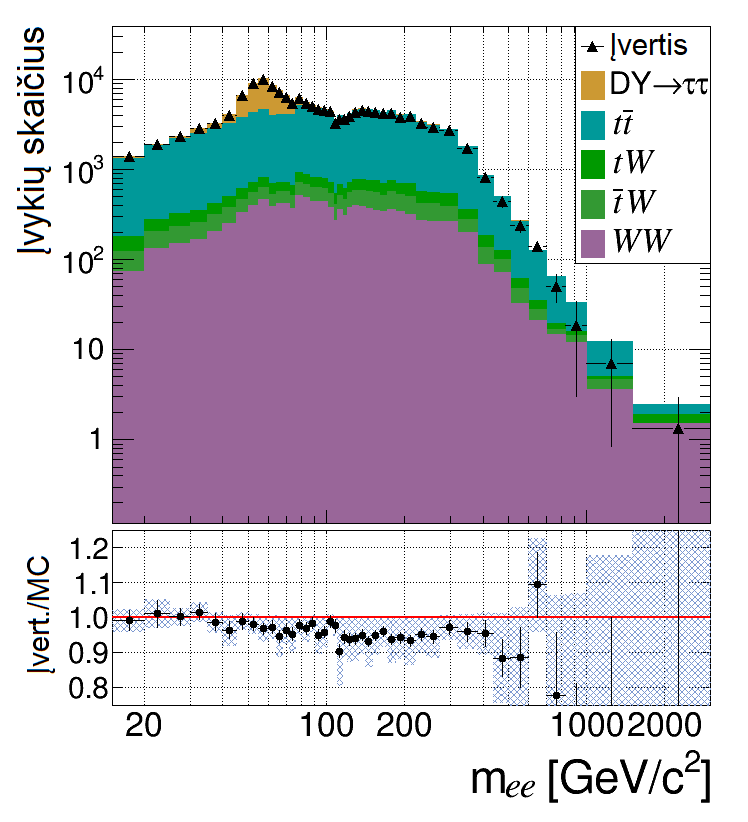
\includegraphics[width=\linewidth]{ee_bkg_est.png}
\end{minipage}
\hfill
\begin{minipage}[t]{0.48\textwidth}
	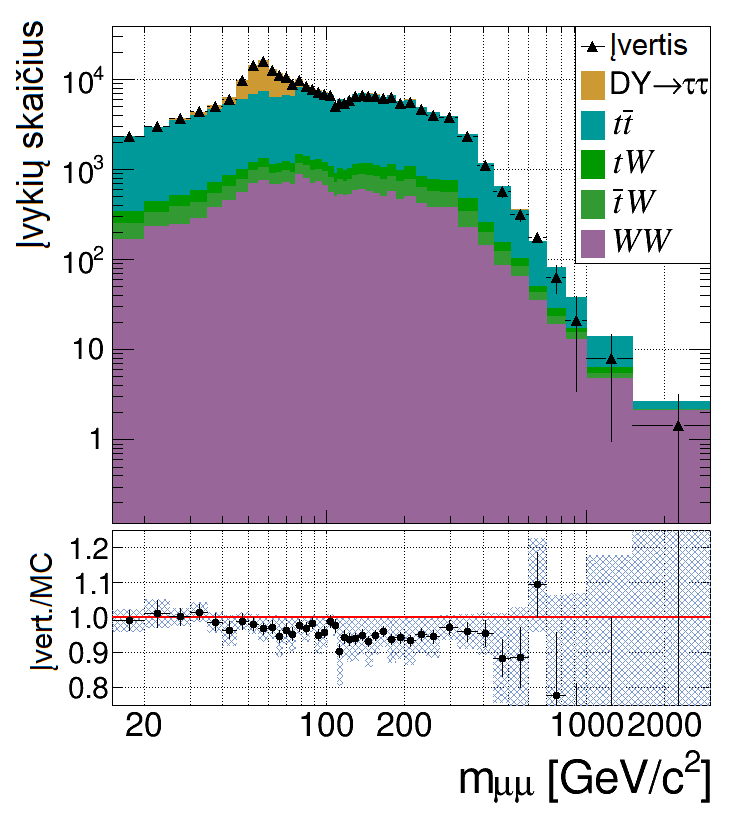
\includegraphics[width=\linewidth]{mumu_bkg_est.png}
\end{minipage}
\vspace{-0.9cm}
\captionof{figure}{\label{fig:bkgEst}
		Su Drell-Yan triukšmo procesais siejamų elektronų (kairėje) ir miuonų (dešinėje) porų invariantinių masių pasiskirstymai.
		Spalvoti histogramų stulpeliai vaizduoja modeliuotus, o juodi taškai -- $\emu$ metodu apskaičiuotus pasiskirstymus.
		Po grafikais pateikiami $\emu$ metodo įverčio ir modeliavimo santykio pasiskirstymai.}
%\vspace{0.9cm}

\noindent\begin{minipage}[t]{0.48\textwidth}
	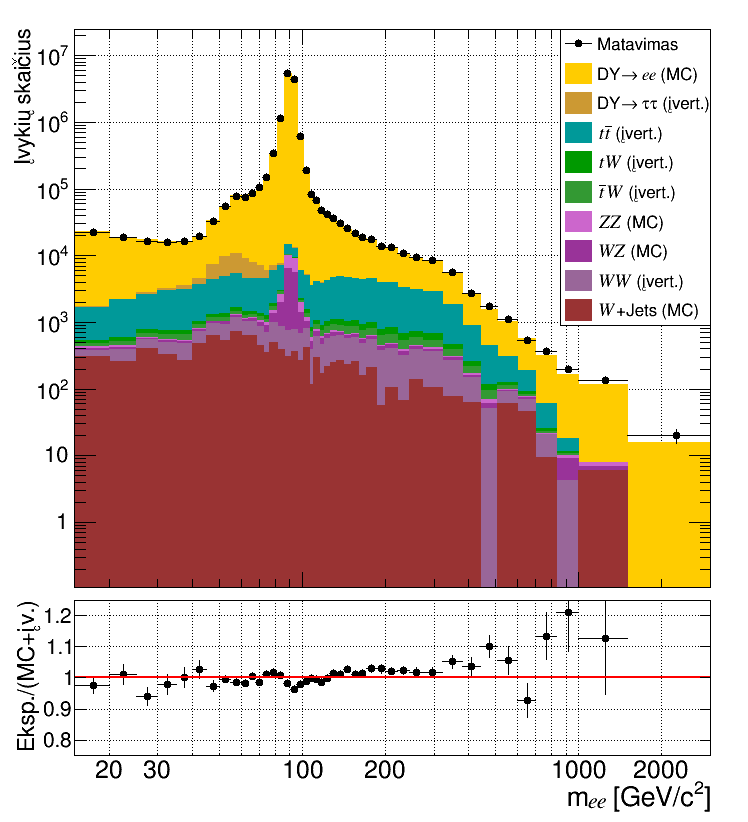
\includegraphics[width=\linewidth]{ee_mass_est.png}
\end{minipage}
\hfill
\begin{minipage}[t]{0.48\textwidth}
	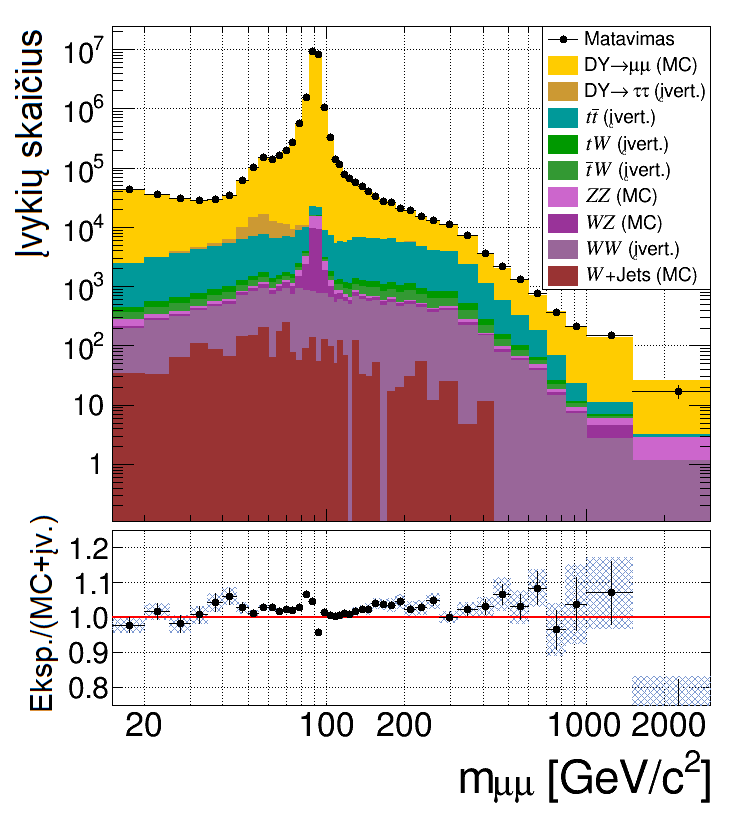
\includegraphics[width=\linewidth]{mumu_mass_est.png}
\end{minipage}
\vspace{-0.9cm}
\captionof{figure}{\label{fig:MassDataMCest}
		Elektronų (kairėje) ir miuonų (dešinėje) porų invariantinių masių pasiskirstymų histogramos, kuriose, kur įmanoma, modeliuotų įvykių skaičius yra
		pakeistas $\emu$ metodu įvertintu įvykių skaičiumi.}
		
\clearpage
\section{Santrauka}
Šiame darbe pristatoma Drell-Yan proceso paieška analizuojant CERN CMS eksperimento 2016 metais užregistruotus
$13$ TeV energijos protonų susidūrimų duomenis duomenis, atitinkančius $35.9$ \invfb integruotąjį šviesį.
Paieška buvo vykdoma elektronų ir miuonų kanaluose.
Įvykdžius į Drell-Yan procesą panašių įvykių atranką buvo bandoma nustatyti, kokį indėlį į atranką praėjusių leptonų
porų invariantinių masių pasiskirstymus įneša triukšmo įvykiai.
$\DYtau$, $t\bar{t}\,$, $WW$, $tW$ ir $\bar{t}W$ procesų indėliai buvo įvertinti matavimu grįstu $\emu$ metodu, o
$ZZ$, $WZ$ ir $W+\mathrm{Jets}$ indėliai buvo nustatyti iš modeliavimo.
$QCD$ proceso įnašas bus nustatomas ateityje.
Elektronams ir miuonams buvo pritaikytos atitinkamai energijos ir skersinio impulso matavimo skalių pataisos.
Taip pat modeliuotiems įvykiams buvo pritaikytas rinkinys pataisų, įskaitančių įvairius neatitikimus tarp eksperimento
ir modeliavimo sąlygų.

\section*{Padėka} \addcontentsline{toc}{section}{Padėka}
Tyrimą finansavo Lietuvos mokslo taryba (sutarties nr.\ 09.3.3-LMT-K-712-10-0128).
Tyrimas buvo įgyvendintas autoriui bendradarbiaujant su tyrėjais iš Seulo nacionalinio universiteto (Pietų Korėja),
Nebraskos-Linkolno universiteto (JAV).

\addcontentsline{toc}{section}{Literatūros sąrašas}
\bibliography{KursinisDarbas}
\bibliographystyle{unsrt}

%\clearpage
%\section*{Terminai} \addcontentsline{toc}{section}{Terminai}

\end{document}